\subsection{Airfoil Analysis}
The desired cruise conditions for the aircraft fall within transonic speed regime.  This provides favorable conditions for the sizing analysis but results in an increase in wave drag force.

\begin{wrapfigure}{r}{0.5\textwidth}
    \centering
    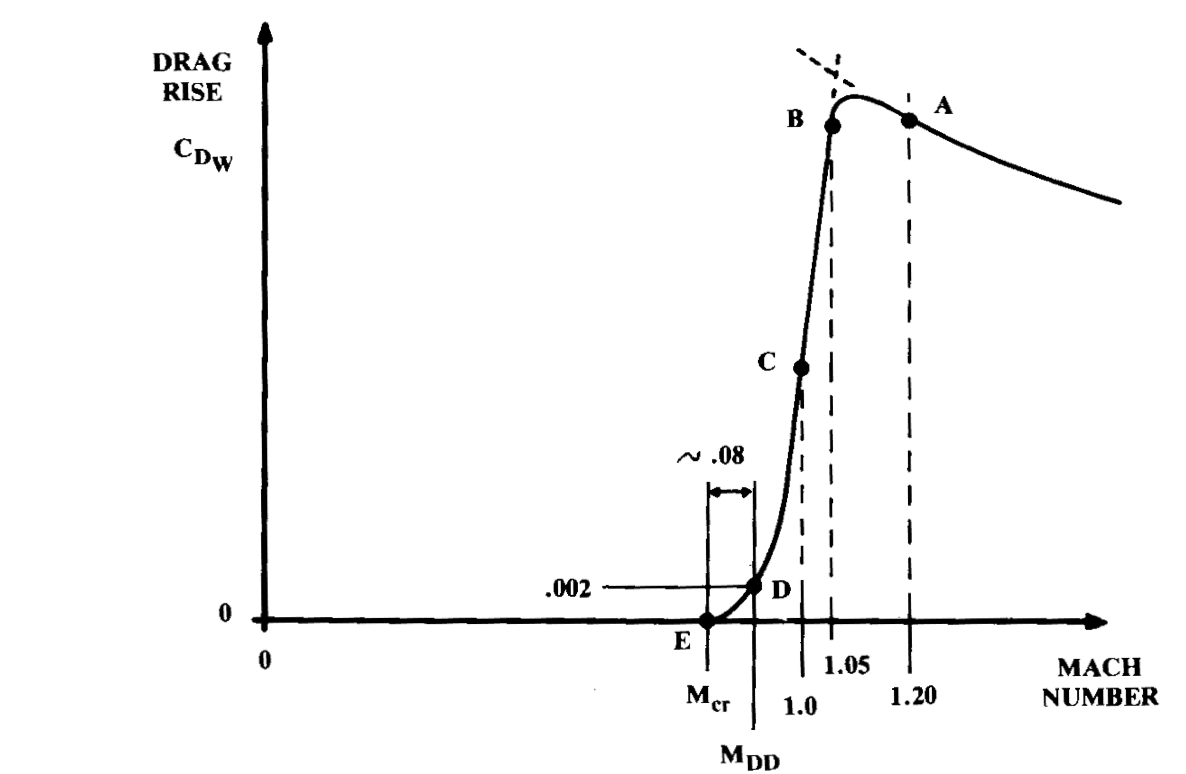
\includegraphics[width=0.5\textwidth]{Photos/wavedragduetotransonic.png}
    \caption{Wave Drag due to Transonic Airspeed\\{\small From Raymer Fig. 12.29\cite{raymer}}}
    \label{fig:transonic}
\end{wrapfigure}

As shown above in figure \ref{fig:transonic}, there is an increase in wave drag as the aircraft passes into the transonic regime.  Therefore, a selection of supercritical airfoils and wing sweep of no less than $30\degree$ is proposed in mitigation of the above trend.  To properly predict and quantify the wave drag for aerodynamic analysis on the airfoil and wing design, the \textit{Delta Method} and \textit{Method B} from Vargas\cite{vargas} shall be included in the part-by-part drag buildup.

\subsection{Wing Design}

\subsection{Drag Buildup}

\subsection{High-Lift Systems}

\subsection{Future Progress}


Will talk about supercritical airfoil analysis, run-through preliminary XFLR5 data, and general drag buildup. - Josh
\textcolor{red}{
\begin{itemize}
    \item Discuss wing design, including reasoning.
    \item Discuss high-lift system, including reasoning.
    \item Discuss drag buildup (tabulated) used to support sizing analysis.
    \item Discuss future work.
    \item AIAA: Important aerodynamic characteristics and aerodynamic performance for key mission
    segments and requirements (shared w/ aero)
\end{itemize}}